\documentclass[11pt,a4paper]{article}
\usepackage[utf8]{inputenc}
\usepackage[T1]{fontenc}
\usepackage{lmodern}
\usepackage[margin=2.3cm]{geometry}
\usepackage{amsmath,amssymb,amsthm,mathtools}
\usepackage{booktabs,multirow,graphicx,xcolor,array}
\usepackage[numbers,sort&compress]{natbib}
\usepackage[colorlinks=true,linkcolor=blue!50!black,citecolor=blue!50!black,urlcolor=blue!50!black]{hyperref}
\usepackage{caption}
\captionsetup{font=small}

\newtheorem{proposition}{Proposition}
\newtheorem{lemma}[proposition]{Lemma}
\newtheorem{corollary}[proposition]{Corollary}
\theoremstyle{definition}
\newtheorem{definition}[proposition]{Definition}
\theoremstyle{remark}
\newtheorem{remark}[proposition]{Remark}
\newcommand{\OWA}{\operatorname{OWA}}
\newcommand{\WOS}{\operatorname{WOS}}
\newcommand{\R}{\mathbb{R}}

\title{Train with Ramps, Deploy with Ranks:\\
Learnable Weighted Order Statistic Cascades as Tiny, Robust,\\ Multiplication-Free Alternatives to Neural Networks}
\author{Juan Carlos del R{\'\i}o\thanks{Independent researcher, Madrid, Spain. \texttt{jcdelrio100@gmail.com}}}
\date{October 2026 \quad (preprint)}

\let\svthefootnote\thefootnote
\begin{document}
\maketitle

\begin{abstract}
Order-statistic filters are increasing, 1-Lipschitz in $\ell_\infty$, have explicit breakdown points and need no
multiplications, but they are hard to train because a selection is piecewise constant in its parameters. We parameterise
cascades of flat weighted order statistic (WOS) filters by real repetition weights and a quantile, train them through a
\emph{ramp} relaxation that spreads each sample's mass between its rank neighbours, which gives exact, non-vanishing
gradients without temperatures, and deploy the \emph{exact} WOS cascade, so every guarantee holds for the deployed model.
When a linear read-out follows the selections, annealing the ramp to the hard selection during training is necessary.
We benchmark the resulting models (WOS-R) against residual convolutional neural networks (CNNs), multilayer perceptrons (MLPs) and small Transformers on five
problems, reporting
accuracy, operator coverage and cost. With 16--137 parameters and at most 8 multiplications per sample, WOS-R comes
within 1.2\,dB of a 22k-parameter CNN on 1D impulsive restoration and beats it when the impulse amplitude doubles, where
a Transformer breaks down. On the BSD68 natural-image test set, a switching WOS-R with 52 parameters is 0.5\,dB behind a 75k-parameter denoising CNN
(DnCNN) at
50\,\% salt-and-pepper noise, and plain WOS-R cascades are 5.6--6.7\,dB ahead of it on random-valued impulses never seen in
training. In radar constant-false-alarm-rate (CFAR) detection, a 34-parameter WOS-R is the best detector in the presence of interfering targets, where an
MLP loses up to 4.3\,dB and a Transformer never reaches a detection probability $P_d=0.5$. In federated aggregation, robustness comes from rank
cascades, not from learned aggregators. The coverage study delineates the class: at 35\,dB signal-to-noise ratio (SNR) the deployed WOS-R recovers median, erosion and
weighted-WOS operators exactly, where all networks remain 5--27\,dB above the noise floor; it fails by construction on
signed linear and level-dependent operators, and ramp training does not always find representable two-stage cascades.
\end{abstract}

%=====================================================================================================
\section{Introduction}
\let\thefootnote\relax\footnotetext{Abbreviations are expanded at first use and listed in Appendix~\ref{app:abbr}.}\addtocounter{footnote}{0}\let\thefootnote\svthefootnote
Rank-order (order-statistic) filters---median, erosion/dilation, weighted medians, stack filters---were a mainstay of
nonlinear signal processing in the 1980s and 1990s because they remove impulses while preserving edges, are
translation invariant and need no multiplications \cite{pitas1990,wendt1986stack,yin1996}. A recurring difficulty was
\emph{design}: superposition does not apply, and early adaptive schemes relied on least-mean-squares (LMS) stochastic gradients through
implicit formulations of the rank operation \cite{salembier1992,pitas1991,ropert1994}. In 1993 the author studied the
adaptation of \emph{cascades} of two order filters \cite{delrio1993}, a problem that is harder than adapting a single
filter because the composition is not reducible to one filter, as it is in the linear case. That work showed that
structures whose parameters act only on the \emph{index} of the selected sample (a binary mask and a rank) cannot be
adapted in cascade, and that structures in which parameters enter the \emph{value} of the selected sample can.

Three decades later, deep networks dominate signal and image restoration, and the questions have changed: how
\emph{small}, \emph{robust} and \emph{cheap} can a learned model be, and what guarantees does it keep? Order-statistic
models are attractive in this regard. They are Lipschitz by construction, they have explicit breakdown points, they
can be implemented with comparators only, and their parameters are interpretable. Their weakness remains
trainability: a selection operator is piecewise constant in its parameters, so gradients vanish almost everywhere.
This is the same ``gradient sparsity'' recently identified for morphological networks \cite{dimitrova2026}.

\paragraph{This paper.} We revisit that problem with modern tools and propose a simple recipe, \emph{train with ramps,
deploy with ranks} (WOS-R):
\begin{enumerate}
\item We parameterise each stage as a flat weighted order statistic (WOS) filter, i.e.\ a filter in which each sample
  of the window enters the sorted list with a real-valued \emph{repetition count} $w_j\ge0$, together with a quantile
  $r$ (Section~\ref{sec:wos}). This is the classical weighted median/WOS family \cite{brownrigg1984,yliharja1991,yin1996},
  and we make its expressiveness precise for cascades.
\item During training only, we replace each repetition by a \emph{ramp} that spreads the sample's mass between the
  mid-points to its rank neighbours (Section~\ref{sec:ramp}). The resulting quantile is continuous and piecewise linear
  in $(w,r)$, so exact gradients exist everywhere without temperatures, straight-through estimators \cite{bengio2013ste}
  or soft sorting \cite{grover2019,blondel2020,petersen2021}. At deployment the ramp is removed and the model is an
  \emph{exact} cascade of selections, so all the guarantees of rank filters apply to the model that is actually used.
\item We benchmark WOS-R against residual convolutional neural networks (CNNs, in the style of the denoising CNN DnCNN
  \cite{zhang2017dncnn}), multilayer perceptrons (MLPs) and small Transformers \cite{liu2021swin} on five problems: 1D impulsive restoration, an operator-coverage matrix (system identification),
  image impulse denoising on the standard Set12 and BSD68 (Berkeley segmentation dataset, 68 images) test sets
  \cite{martin2001bsd}, radar constant-false-alarm-rate (CFAR) detection in K-distributed sea clutter
  \cite{rohling1983,ward2013}, and Byzantine/fault-robust aggregation in federated learning (FL; training distributed over nodes, some of them
  faulty or malicious) \cite{yin2018byz,karimireddy2021,allouah2023}. We report accuracy, \emph{coverage} (which operator classes each model
  can and cannot represent) and cost: parameters, multiplications and comparisons per output sample, and CPU latency.
\end{enumerate}

\paragraph{Contributions.}
(i) A training recipe for exact WOS cascades: repetition weights plus a ramp relaxation used only during training, with
ramp continuation when a linear read-out follows (Sections~\ref{sec:wos}--\ref{sec:ramp}).
(ii) Properties of the deployed model: integer equivalence, class-$\mathcal O$ Lipschitz bound independent of depth,
breakdown point as a function of the repetitions, and a Matheron--Maragos test of when a cascade collapses to one WOS.
(iii) A benchmark of accuracy, coverage and cost against CNN, MLP and Transformer baselines on five problems, with all
code and result files (Section~\ref{sec:results}).
(iv) A delimitation of where order-statistic models are preferable---impulsive and heavy-tailed contamination,
out-of-distribution amplitudes and contamination types, interference-limited detection, Byzantine aggregation, and
multiplication-free hardware---and where they are not---Gaussian noise in distribution, signed linear operators and
contamination rates beyond the design breakdown point (Section~\ref{sec:disc}).

%=====================================================================================================
\section{Related work}
\paragraph{Order-statistic and stack filters.} Weighted median and WOS filters \cite{brownrigg1984,yin1996} are stack
filters \cite{wendt1986stack} whose Boolean function is a threshold function \cite{yliharja1991}. Arce's weighted
median admits negative weights \cite{arce1998}. Adaptive design used LMS-type or sigmoidal approximations
\cite{salembier1992,pitas1991,ropert1994,yin1996} and, later, support vector machines (SVMs) on the threshold decomposition \cite{yao2006}.
Salembier's adaptive rank-order filters \cite{salembier1992} and their cascades \cite{delrio1993} are the direct
ancestors of this work.
\paragraph{Morphological and tropical networks.} Morphological perceptrons \cite{ritter1996,charisopoulos2017}, smooth
morphological layers \cite{hermary2022}, sparse hybrid linear--morphological networks \cite{fotopoulos2025} and the tropical
view of ReLU networks \cite{zhang2018tropical} relate max-plus algebra to deep learning. Training difficulties are
attributed to gradient sparsity and initialisation sensitivity \cite{dimitrova2026}. Sorting-based activations also
yield Lipschitz networks \cite{anil2019}.
\paragraph{Differentiable sorting.} NeuralSort \cite{grover2019}, projection-based soft sort/rank \cite{blondel2020} and
differentiable sorting networks \cite{petersen2021} relax \emph{permutations}. Our ramp relaxes the \emph{quantile of a
weighted empirical distribution}, is exact at deployment ($\beta=0$), and leaves the sorting itself hard.
\paragraph{Robust aggregation and CFAR.} Coordinate-wise median and trimmed mean \cite{yin2018byz}, Krum
\cite{blanchard2017}, centred clipping \cite{karimireddy2021} and nearest-neighbour mixing \cite{allouah2023} are
order-statistic aggregators facing attacks such as ``a little is enough'' (ALIE, small coordinated shifts hidden within
the honest spread) \cite{baruch2019} and inner-product manipulation (IPM, updates that reverse the sign of the honest
mean's inner product) \cite{xie2019ipm}. Order-statistic CFAR (OS-CFAR, threshold from the $k$-th ranked reference cell)
\cite{rohling1983} and its greatest-of/smallest-of (GO/SO) variants \cite{gandhi1988} are rank-filter detectors.

%=====================================================================================================
\section{Weighted order statistic cascades}\label{sec:wos}
\subsection{Definitions}
Let $z\in\R^m$ be the window of a signal or image around the current sample, $w\in\R_{\ge0}^m$ the repetition weights,
$W=\sum_jw_j$ and $r\in(0,1)$. The WOS output is the lower weighted $r$-quantile
\begin{equation}\label{eq:wos}
\WOS_{w,r}(z)=\min\Big\{z_{(k)}:\ \textstyle\sum_{j:\,z_j\le z_{(k)}}w_j\ \ge\ rW\Big\}.
\end{equation}
For $w\in\mathbb N^m$ this is exactly ``sort the list in which $z_j$ appears $w_j$ times and take position $\lceil rW\rceil$''.
$w_j=0$ removes the tap (a mask); $w\equiv1$ gives the rank filters, and $r\to0$, $r\to1$ give erosion and dilation.
A WOS-R model is a \emph{cascade} of WOS stages, or a \emph{bank} of $C$ cascades combined by an affine mix
$y=\sum_c a_cy_c+b$. The mix contributes the only $C$ multiplications per output sample.

\subsection{Properties}
\begin{proposition}[repetitions, thresholds and integers]\label{prop:thr}
(i) $(\lambda w,r)$ and $(w,r)$ define the same filter for all $\lambda>0$.
(ii) By threshold decomposition, $\WOS_{w,r}(z)\ge t$ iff $\sum_{j:z_j\ge t}w_j>(1-r)W$: a positive threshold Boolean function.
(iii) Every real-weight WOS equals an integer-weight WOS, because there are finitely many threshold functions of $m$ variables.
\end{proposition}

\begin{proposition}[class $\mathcal O$ and Lipschitz]\label{prop:lip}
Every flat WOS cascade (and every cascade of ordered weighted averages, OWA $\sum_kw_kz_{(k)}$, including the 1993
NEst structure $\sum_k|h_k|(z+b)_{(k)}$, with weights in the simplex) is increasing, commutes with translations
and satisfies $\Psi(z+c)=\Psi(z)+c$. Consequently $\|\Psi(x)-\Psi(y)\|_\infty\le\|x-y\|_\infty$, independently of depth.
\end{proposition}
\begin{proof}
If $x\le y+\delta$, then $\Psi x\le\Psi(y+\delta)=\Psi y+\delta$; exchange $x$ and $y$.
\end{proof}

\begin{proposition}[breakdown]\label{prop:bp}
A set $S$ of arbitrarily corrupted window samples can drive $\WOS_{w,r}$ to $\pm\infty$ iff
$w(S)\ge\min\{\lceil rW\rceil,\,W-\lceil rW\rceil+1\}$. Boosting the weight of a position therefore \emph{reduces} the
number of corrupted samples needed: for a 5-point median with centre weight 3, two samples suffice instead of three.
\end{proposition}

\begin{proposition}[Matheron--Maragos basis]\label{prop:basis}
Every flat cascade is $\Psi z=\max_{B\in\mathcal B}\min_{b\in B}z_b$, where $\mathcal B$ is the set of minimal true sets
of its Boolean function \cite{matheron1975,maragos1989}. A rank-$r$ filter of $m$ samples needs $\binom{m}{m-r+1}$
erosions, against $m{+}1$ WOS parameters. A cascade is a single WOS iff its Boolean function is a threshold function;
a mixed-integer linear program on the truth table decides this and returns the minimal integer repetitions.
\end{proposition}
On the 20 two-stage cascades used in our experiments, 8 are single WOS (verified with zero error), while openings,
median-of-medians and the cascade studied in 1993 are not. This motivates cascades and banks.

%=====================================================================================================
\section{The ramp relaxation}\label{sec:ramp}
\begin{definition}[ramp WOS]
Sort $z$ and let $m_k^-=z_{(k)}-\beta\frac{z_{(k)}-z_{(k-1)}}2$ and $m_k^+=z_{(k)}+\beta\frac{z_{(k+1)}-z_{(k)}}2$
(extremes are not extended), with $\beta\in[0,1]$. Sample $k$ carries mass $w_{(k)}$ spread uniformly over
$[m_k^-,m_k^+]$. The ramp-WOS output is the $r$-quantile of this piecewise-linear distribution:
\begin{equation}\label{eq:ramp}
y=m^-_{k^*}+\frac{rW-C_{k^*-1}}{w_{(k^*)}}\,\big(m^+_{k^*}-m^-_{k^*}\big),\qquad k^*=\min\{k:C_k\ge rW\},\quad C_k=\textstyle\sum_{i\le k}w_{(i)}.
\end{equation}
The integer version places $w_{(k)}$ equispaced points in $[m_k^-,m_k^+]$; for example $(0,1),(0.5,3),(1,1)$ yields the
list $[0,\,0.25,\,0.5,\,0.75,\,1]$.
\end{definition}

\begin{proposition}\label{prop:ramp}
(i) $\beta=0$ recovers \eqref{eq:wos} exactly.
(ii) For $\beta=1$ the cells tile $[z_{(1)},z_{(m)}]$, so $y$ is continuous and piecewise linear in $(w,r)$, with
$\partial y/\partial r$ and $\partial y/\partial w$ defined almost everywhere and non-zero on a set of positive measure.
(iii) With uniform weights and $r=\tfrac12$ (odd $m$), the ramp median is the L-filter $\tfrac14z_{(k-1)}+\tfrac12z_{(k)}+\tfrac14z_{(k+1)}$.
(iv) With non-uniform weights, the ramp is \emph{not} continuous in $z$: swapping two samples with different weights
re-assigns cells. It is neither increasing nor 1-Lipschitz, and its breakdown point drops by one rank neighbour.
\end{proposition}
Property (iv) is why we use the ramp \emph{only for training}. The deployed model ($\beta=0$) is an exact WOS cascade and
satisfies Propositions~\ref{prop:lip}--\ref{prop:basis}. Table~\ref{tab:props} quantifies (ii) and (iv).

\begin{table}[t]\centering\small
\caption{Measured properties with non-uniform weights $w=(1,2,3,1,0.5,2,1)$, $r=0.4$, on $2\cdot10^4$ random windows of 7 samples. ``Jump in $r$'': largest output change when $r$ moves by $5\cdot10^{-3}$. Last two columns: largest output magnitude of the 5-point (ramp) median with uniform weights under $k$ impulses of $10^6$.}\label{tab:props}
\resizebox{\linewidth}{!}{\begin{tabular}{lcccccc}\toprule
Operator & Increasing & $\Psi(z{+}c){=}\Psi(z){+}c$ & Lipschitz $\ell_\infty$ & Jump in $r$ & 2 impulses & 3 impulses\\\midrule
Exact WOS ($\beta=0$) & yes & yes & 1.00 & 3.46 & 3.9 & $1.0\cdot10^{6}$\\
Ramp, $\beta=1$ & \textbf{no} & yes & 5.73 & 0.17 & $2.5\cdot10^{5}$ & $7.5\cdot10^{5}$\\
Ramp, $\beta=0.5$ & \textbf{no} & yes & 3.88 & 1.78 & -- & --\\
Ramp, integer version & \textbf{no} & yes & 9.14 & -- & 3.9 & $1.0\cdot10^{6}$\\
\bottomrule\end{tabular}}\end{table}

\begin{remark}[ramp continuation for linear read-outs]\label{rem:cont}
For a pure cascade, the ramp's interpolation error is a common-mode bias that the discrete parameters cannot absorb, and
the deployed selection snaps to the right order statistic: in our coverage experiment the ramp-trained chain has an
excess error of 18.5--21.6\,dB at $\beta=1$ and 0.0\,dB \emph{after deployment} on every single-WOS target
(Table~\ref{tab:b2}). When a linear layer follows the selections (the affine mix of a bank), the mix can co-adapt to the
ramp, combining slightly different quantiles into an interpolation that disappears at $\beta=0$; a ramp-only bank then
misses even a 7-point median by 20\,dB. Annealing $\beta$ linearly from 1 to 0 during training (we use the first 70\,\% of
the steps) removes the effect; refitting the mix by least squares after training does not, because the chains
themselves have co-adapted. We therefore train chains with $\beta=1$ and banks with this ramp continuation.
\end{remark}

\paragraph{Why it helps.} With the exact WOS, $\partial y/\partial w=\partial y/\partial r=0$ almost everywhere. The
straight-through alternative uses the gradient of a temperature-smoothed cumulative distribution function (CDF) evaluated at the hard output; the soft
alternative anneals a temperature. The ramp provides the exact gradient of a nearby continuous model whose distance to
the deployed WOS is bounded by half the local spacing of the order statistics.

%=====================================================================================================
\section{Experimental protocol}\label{sec:proto}
All experiments run on a 2-core CPU with PyTorch. WOS-R stages are trained with Adam ($\eta=0.03$, cosine schedule) at
$\beta=1$ (banks: $\beta$ annealed $1\to0$ over the first 70\,\% of the steps, Remark~\ref{rem:cont}) and evaluated at
$\beta=0$; baselines use Adam ($\eta=10^{-3}$ or $2\cdot10^{-3}$) with the same data, loss
(mean squared error, MSE) and number of steps. ``Mults'' counts multiply--accumulates per output sample (attention included),
``Comps'' counts comparisons for sorting (bound $m\lceil\log_2m\rceil$ per stage), and latency is single-threaded CPU
time. Exact configurations are listed in Appendix~\ref{app:hyper}; the code and all result files are released with the paper.

%=====================================================================================================
\section{Results}\label{sec:results}

\subsection{B1: one-dimensional restoration}
Table~\ref{tab:b1} reports restoration of piecewise-smooth 1D signals, measured by the normalised mean squared error
(NMSE $=\|\hat s-s\|^2/\|s\|^2$ in dB; lower is better). Under impulsive noise, a two-stage WOS-R chain with
16 parameters and no multiplications reaches $-20.5$\,dB, better than the 3\,857-parameter medium CNN (CNN-M; S/M/L denote
small/medium/large) ($-19.4$\,dB), the MLP
($-19.9$\,dB) and the Transformer ($-18.5$\,dB). These three runs are, however, favourable for the single chain: over 20 independent trainings (B1, the convergence study and the restart study in the released code) it reaches $-18.7\pm1.3$\,dB (range $-20.7$ to $-16.9$), and keeping the best of 4 restarts selected on validation data gives $-19.6$\,dB, on a par with CNN-M. Banks are far less sensitive to initialisation ($-21.1\pm0.5$\,dB over 6 runs for $C{=}8$). The bank with $C{=}8$ chains (137 parameters, 8 multiplications per
sample) reaches $-21.1$\,dB, 1.2\,dB behind the best model, CNN-L, which uses 161 times more parameters and 2\,744 times
more multiplications. When the impulse amplitude doubles (out of distribution, OOD $\times2$), the ordinal models degrade least: WOS-R bank
$C{=}8$ ($-17.8$\,dB) and the 1993 NEst bank ($-18.2$\,dB) overtake CNN-L ($-17.4$\,dB), while the Transformer breaks
down ($+0.3$\,dB, against $+9.7$\,dB for the noisy input), as Proposition~\ref{prop:lip} would predict for a model that is
not 1-Lipschitz. When the impulse \emph{rate} increases to 25\,\%, the CNNs extrapolate better ($-15.5$ vs $-12.4$\,dB):
a WOS cascade designed for 10\,\% contamination has a fixed breakdown point (Prop.~\ref{prop:bp}).

Under Gaussian noise, averaging is required and CNNs win in distribution ($-20.4$ vs $-18.2$\,dB); at twice the noise
level the ranking reverses and WOS-R bank $C{=}8$ is the best model ($-12.7$\,dB vs $-11.6$\,dB for CNN-L). Ramp
continuation improves the banks by 0.9--1.5\,dB over ramp-only training (ablation rows), consistently with
Remark~\ref{rem:cont}. Keeping the ramp at test time ($\beta=1$) is 0.9--1.3\,dB \emph{worse} under impulses in
distribution (0.3--1.4\,dB over all impulsive columns) but 1.0\,dB better for the Gaussian chain, because the $\beta=1$ ramp median is an L-filter (Prop.~\ref{prop:ramp}(iii)); we keep
$\beta=0$ throughout for the guarantees.

\begin{table*}[t]\centering\small
\caption{B1: 1D restoration, normalised mean squared error (NMSE) in dB (mean $\pm$ std over 3 seeds; lower is better). Impulsive models are trained with 10\,\% impulses; OOD (out-of-distribution) columns change impulse rate or amplitude. NEst: 1993 thesis structure; CNN-S/M/L: small/medium/large residual CNN. Gaussian models are trained with $\sigma=0.2$. Params, multiply--accumulates and comparisons per output sample; ms: CPU latency for 4096 samples (1 thread). Best per column in bold.}\label{tab:b1}
\resizebox{\linewidth}{!}{\begin{tabular}{lrrrr|ccc|cc}\toprule
& & & & & \multicolumn{3}{c|}{Impulsive} & \multicolumn{2}{c}{Gaussian}\\
Model & Params & Mults & Comps & ms & in-dist & OOD $p{=}25\%$ & OOD $\times2$ & $\sigma{=}0.2$ & $\sigma{=}0.4$ (OOD)\\\midrule
Median 5 & 0 & 0 & 15 & 0.3 & $-13.7\pm1.2$ & $-3.6\pm0.3$ & $-8.0\pm1.3$ & $-14.9\pm0.3$ & $-8.9\pm0.4$\\
WOS-R chain $2{\times}7$ & 16 & 0 & 42 & 2.1 & $-20.5\pm0.1$ & $-11.3\pm0.3$ & $-16.5\pm1.7$ & $-16.4\pm0.3$ & $-11.1\pm0.4$\\
WOS-R bank $C{=}4$ & 69 & 4 & 168 & 7.8 & $-20.8\pm0.5$ & $-12.1\pm0.5$ & $-17.4\pm1.1$ & $-17.9\pm0.2$ & $-12.4\pm0.4$\\
WOS-R bank $C{=}8$ & 137 & 8 & 336 & 16.9 & $-21.1\pm0.6$ & $-12.4\pm0.6$ & $-17.8\pm0.9$ & $-18.2\pm0.4$ & $\mathbf{-12.7\pm0.4}$\\
\quad ablation: bank $C{=}4$, ramp only & 69 & 4 & 168 & 7.8 & $-19.9\pm0.9$ & $-11.1\pm1.6$ & $-16.1\pm1.4$ & -- & --\\
\quad ablation: bank $C{=}8$, ramp only & 137 & 8 & 336 & 16.9 & $-19.8\pm0.9$ & $-10.9\pm1.7$ & $-16.5\pm1.2$ & -- & --\\
NEst bank $C{=}4$ & 117 & 60 & 168 & 3.7 & $-21.0\pm0.4$ & $-12.3\pm0.3$ & $\mathbf{-18.2\pm0.9}$ & $-18.5\pm0.2$ & $-12.5\pm0.3$\\
CNN-S & 129 & 120 & 0 & 0.1 & $-15.0\pm0.7$ & $-8.3\pm0.2$ & $-9.4\pm0.9$ & $-19.1\pm0.3$ & $-11.3\pm0.3$\\
CNN-M & 3\,857 & 3\,808 & 0 & 0.7 & $-19.4\pm0.4$ & $-12.9\pm1.0$ & $-14.6\pm0.6$ & $-20.4\pm0.3$ & $-12.1\pm0.6$\\
CNN-L & 22\,081 & 21\,952 & 0 & 3.8 & $\mathbf{-22.3\pm0.6}$ & $\mathbf{-15.5\pm0.7}$ & $-17.4\pm0.0$ & $\mathbf{-20.4\pm0.2}$ & $-11.6\pm0.7$\\
MLP (window 15) & 5\,249 & 5\,120 & 0 & 1.5 & $-19.9\pm0.3$ & $-12.9\pm0.5$ & $-15.0\pm0.1$ & $-19.7\pm0.3$ & $-12.5\pm0.4$\\
Transformer & 4\,561 & 69\,728 & 0 & 141.0 & $-18.5\pm0.3$ & $-11.1\pm0.2$ & $0.3\pm0.3$ & $-16.5\pm0.3$ & $-9.6\pm0.4$\\
\bottomrule\end{tabular}}\end{table*}

\subsection{B2: coverage}
Table~\ref{tab:b2} probes coverage by system identification at high SNR (35\,dB), where approximate emulation is
penalised. Each cell is the excess error of the deployed model over the noise floor of the true operator; Fig.~\ref{fig:b2}
shows the same data as a map. Four facts stand out.

(i) \emph{Exactness.} When the ramp-trained WOS-R finds the target, it finds it \emph{exactly}: 0.0\,dB on the 7-point
median, the flat erosion, the weighted WOS and rank cascade \#1, for both seeds and both architectures. No network
reaches the floor on any rank-type target: the MLP, CNN-M and Transformer stay 5.5--26.8\,dB above it, i.e.\ they
approximate sorting but do not represent it, with 56--328 times more parameters.

(ii) \emph{Optimisation, not representation, is the bottleneck inside the class.} The opening and rank cascades \#12 and
\#5 are two-stage rank cascades, hence exactly representable by the WOS-R chain, yet ramp training does not find them
(12--25\,dB). This agrees with the identification rate of 9/16 random cascades reported earlier. The 1993 NEst bank,
whose parameters act on values, finds the opening (1.2\,dB) and cascade \#1 but misses the weighted WOS (22.4\,dB): the two
parameterisations fail on different targets.

(iii) \emph{Outside the class.} A flat WOS cascade is increasing and commutes with level shifts
(Prop.~\ref{prop:lip}), so it cannot represent the signed high-pass, the point-wise square or the top-hat; the
bank's affine mix could in principle express the top-hat as identity minus opening, but inherits the failure to find
the opening. Moving averages are not selections either; the bank approaches them only coarsely (22.8\,dB). Networks
represent these operators well (0.1--2.3\,dB for the linear ones).

(iv) \emph{The deployed model, not the relaxed one.} At $\beta=1$ the same trained models are 17--31\,dB above the floor on
every target; the exact selections appear only at $\beta=0$. Ramp training is a means to find the discrete model, not
an approximation used at inference.

\begin{figure}[t]\centering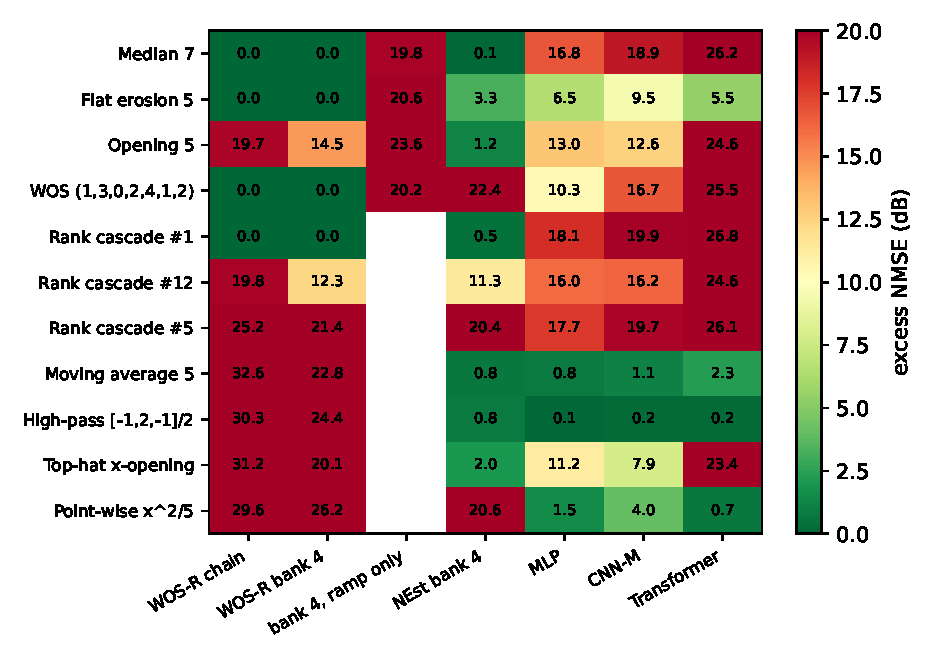
\includegraphics[width=0.68\linewidth]{figs/b2_coverage.pdf}
\caption{Coverage map (excess NMSE above the floor, dB; green: represented, red: not represented).}\label{fig:b2}\end{figure}

\begin{table}[t]\centering\small
\caption{B2 coverage: excess normalised mean squared error (NMSE, dB) above the noise floor of the true operator (input $U[-5,5]$, SNR 35\,dB, mean of 2 seeds). Bold: $\le1$\,dB (operator represented); red: $>6$\,dB (not represented). Parameters in the last row.}\label{tab:b2}
\setlength{\tabcolsep}{4pt}\resizebox{\linewidth}{!}{\begin{tabular}{llrrrrrrr}\toprule
Target & Class & WOS-R chain & WOS-R bank 4 & bank 4, ramp only & NEst bank 4 & MLP & CNN-M & Transformer\\\midrule
Median 7 & rank & \textbf{0.0} & \textbf{0.0} & \textcolor{red!70!black}{19.8} & \textbf{0.1} & \textcolor{red!70!black}{16.8} & \textcolor{red!70!black}{18.9} & \textcolor{red!70!black}{26.2}\\
Flat erosion 5 & morphological & \textbf{0.0} & \textbf{0.0} & \textcolor{red!70!black}{20.6} & 3.3 & \textcolor{red!70!black}{6.5} & \textcolor{red!70!black}{9.5} & 5.5\\
Opening 5 & morph., 2 stages & \textcolor{red!70!black}{19.7} & \textcolor{red!70!black}{14.5} & \textcolor{red!70!black}{23.6} & 1.2 & \textcolor{red!70!black}{13.0} & \textcolor{red!70!black}{12.6} & \textcolor{red!70!black}{24.6}\\
WOS $(1,3,0,2,4,1,2)$ & WOS & \textbf{0.0} & \textbf{0.0} & \textcolor{red!70!black}{20.2} & \textcolor{red!70!black}{22.4} & \textcolor{red!70!black}{10.3} & \textcolor{red!70!black}{16.7} & \textcolor{red!70!black}{25.5}\\
Rank cascade \#1 & rank cascade & \textbf{0.0} & \textbf{0.0} & -- & \textbf{0.5} & \textcolor{red!70!black}{18.1} & \textcolor{red!70!black}{19.9} & \textcolor{red!70!black}{26.8}\\
Rank cascade \#12 & rank cascade & \textcolor{red!70!black}{19.8} & \textcolor{red!70!black}{12.3} & -- & \textcolor{red!70!black}{11.3} & \textcolor{red!70!black}{16.0} & \textcolor{red!70!black}{16.2} & \textcolor{red!70!black}{24.6}\\
Rank cascade \#5 & rank cascade & \textcolor{red!70!black}{25.2} & \textcolor{red!70!black}{21.4} & -- & \textcolor{red!70!black}{20.4} & \textcolor{red!70!black}{17.7} & \textcolor{red!70!black}{19.7} & \textcolor{red!70!black}{26.1}\\
Moving average 5 & linear, $h\ge0$ & \textcolor{red!70!black}{32.6} & \textcolor{red!70!black}{22.8} & -- & \textbf{0.8} & \textbf{0.8} & 1.1 & 2.3\\
High-pass $[-1,2,-1]/2$ & linear, signed & \textcolor{red!70!black}{30.3} & \textcolor{red!70!black}{24.4} & -- & \textbf{0.8} & \textbf{0.1} & \textbf{0.2} & \textbf{0.2}\\
Top-hat $x-$opening & non-increasing & \textcolor{red!70!black}{31.2} & \textcolor{red!70!black}{20.1} & -- & 2.0 & \textcolor{red!70!black}{11.2} & \textcolor{red!70!black}{7.9} & \textcolor{red!70!black}{23.4}\\
Point-wise $x^2/5$ & not translation-inv. & \textcolor{red!70!black}{29.6} & \textcolor{red!70!black}{26.2} & -- & \textcolor{red!70!black}{20.6} & 1.5 & 4.0 & \textbf{0.7}\\
\midrule Params & & 16 & 69 & 69 & 117 & 5\,249 & 3\,857 & 4\,561\\
\bottomrule\end{tabular}}\end{table}

\subsection{B3: image impulse denoising}
Table~\ref{tab:b3bsd68} reports blind impulse denoising on BSD68 (Set12 in Appendix~\ref{app:tables}). All learned models are
trained on salt-and-pepper (SP) noise with random density in $[0.1,0.6]$; random-valued impulses (RVIN) are never seen
in training. Three regimes appear.

Quality is measured by the peak signal-to-noise ratio (PSNR, dB) and the structural similarity index (SSIM, 0--1).
\emph{In distribution}, the best model is DnCNN-M, the 10-layer DnCNN (74\,593 parameters, 74\,304 multiplications per pixel). A
\emph{switching} WOS-R, which applies a learned $5{\times}5$ two-stage WOS cascade only to pixels that are an extreme of
their $3{\times}3$ neighbourhood, reaches 26.22\,dB at SP\,50\,\% (0.52\,dB behind DnCNN-M) with 52 parameters and no
multiplications, has a higher SSIM (0.840 vs 0.761), matches the 17-layer DnCNN (26.20\,dB) and beats the window
Transformer (24.92\,dB). The hand-designed adaptive median filter (AMF) remains a remarkably strong baseline for SP noise
(26.02\,dB at 50\,\%, best SSIM at 70\,\%); the switching WOS-R matches it between 30\,\% and 50\,\% and is 1.6--1.8\,dB
behind at the extremes of the density range.

\emph{Out of distribution} (RVIN), every model that relies on detecting extreme values collapses: AMF, the switching
WOS-R, the MLP, the DnCNNs and the Transformer all fall to 16--19.5\,dB at RVIN\,40\,\%. The plain (non-switching) WOS-R
cascades keep 23.4--24.5\,dB, \emph{5.6--6.7\,dB above DnCNN-M}, because a selection with a bounded breakdown point does not
care whether an outlier is at 0, 1 or anywhere in between. Figure~\ref{fig:qual} shows both effects.

\emph{Gaussian noise} (Table~\ref{tab:b3g}) is outside the natural class of order statistics: on BSD68, WOS-R banks are 2.1--2.4\,dB
behind DnCNN-M at the training level $\sigma=25$, but 4.0--4.6\,dB \emph{ahead} at $\sigma=50$ (Set12: 2.4--2.7 and 4.3--4.9\,dB), where every convolutional
model over-fits its training noise level. In 2D, ramp continuation and ramp-only training give banks within 0.7\,dB of each
other, without a consistent sign; the co-adaptation of Remark~\ref{rem:cont} matters at high SNR (B2) and in 1D (B1).

DnCNN-17 without batch normalisation did not train in our CPU budget (17.06\,dB on Set12 at SP\,10\,\%); we report the
original design with batch normalisation, which after 2\,000 steps is still below the 10-layer DnCNN-M. Our DnCNNs are
therefore \emph{under-trained} relative to the published model \cite{zhang2017dncnn}, and the in-distribution gaps above
are lower bounds on what a GPU-trained network achieves; the OOD collapses are not an artefact of under-training, since
they affect every network regardless of its in-distribution quality.

\begin{figure*}[t]\centering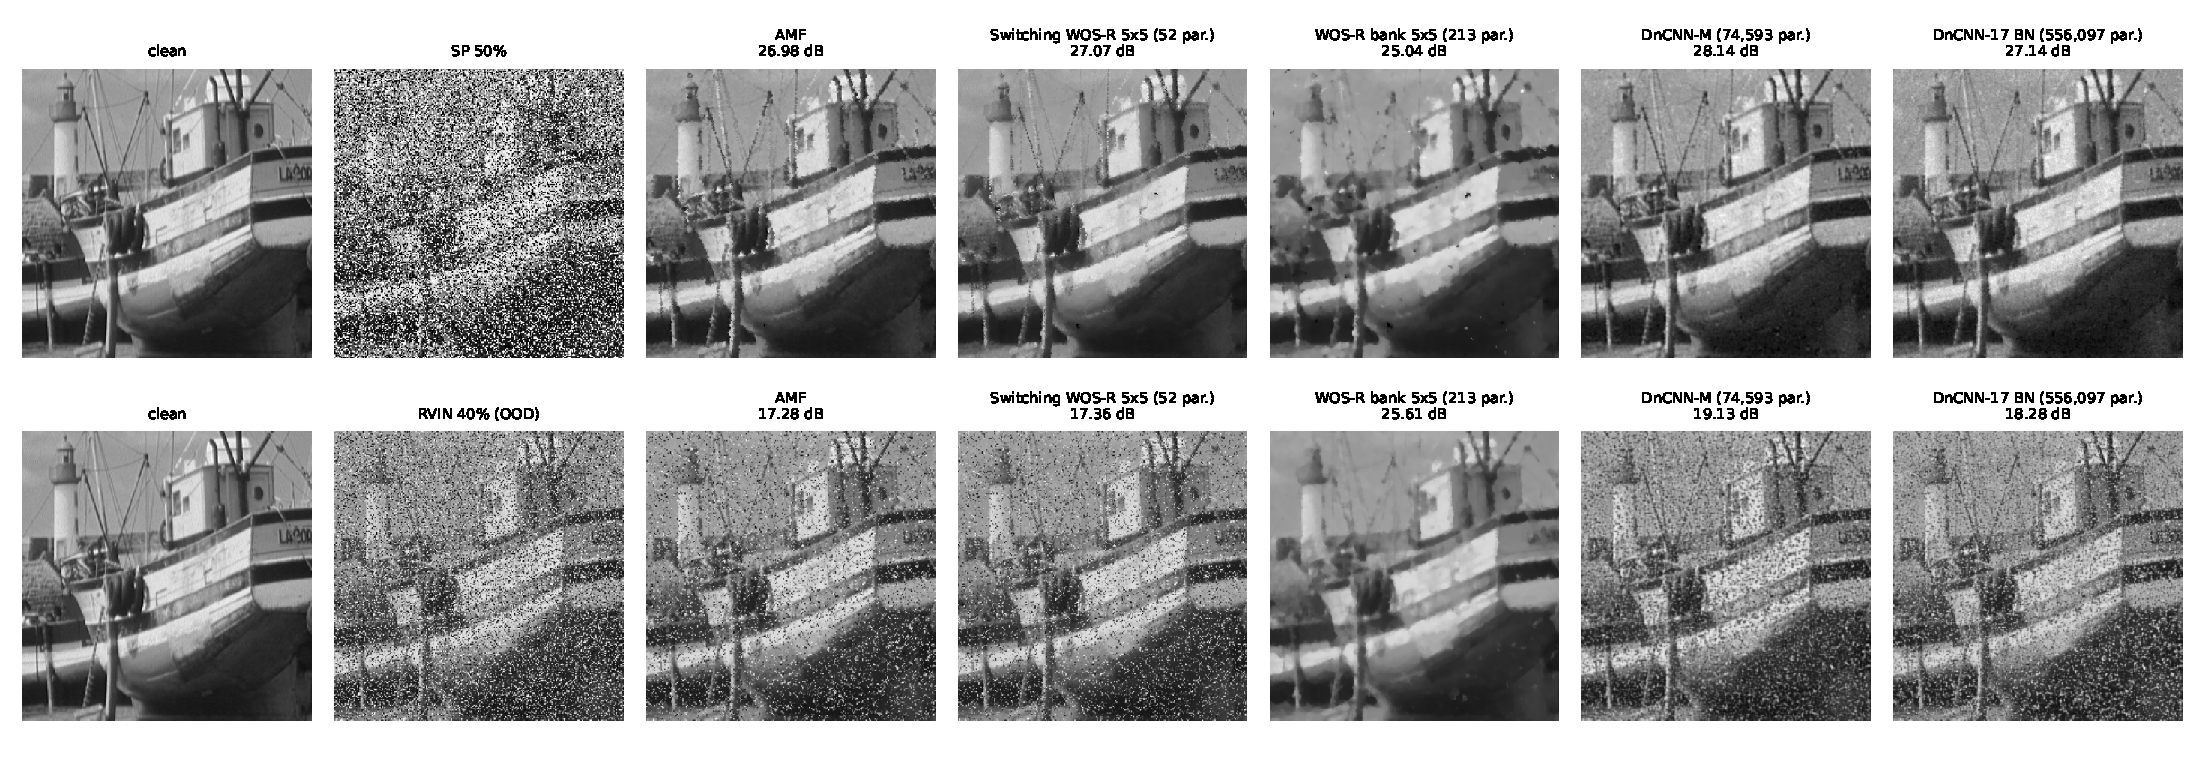
\includegraphics[width=\linewidth]{figs/qual.pdf}
\caption{Set12 ``boat'' ($256{\times}256$ crop; PSNR of the full image). Top: SP 50\,\% (in distribution). Bottom: RVIN
40\,\% (never seen in training). The switching WOS-R matches AMF and approaches DnCNN-M on SP; the plain (non-switching) WOS-R removes
random-valued impulses, which every detection-based model and every network misses.}\label{fig:qual}\end{figure*}

\begin{table}[t]\centering\small
\caption{B3 coverage check: Gaussian denoising (trained at $\sigma=25$), PSNR in dB, Set12 / BSD68. Order statistics are not the right tool here (Prop.~\ref{prop:lip}: no averaging).}\label{tab:b3g}
\begin{tabular}{lrcc}\toprule Model & Params & $\sigma=25$ & $\sigma=50$ (OOD)\\\midrule
Median $3{\times}3$ & 0 & 25.45 / 24.89 & 21.06 / 20.92\\
WOS-R bank $C{=}4$ ($3{\times}3$) & 85 & 26.64 / 26.15 & 21.95 / 21.84\\
WOS-R bank $C{=}4$ ($5{\times}5$) & 213 & 27.00 / 26.45 & 22.56 / 22.42\\
MLP $5{\times}5$ & 5\,889 & 28.19 / 27.59 & 19.88 / 20.00\\
DnCNN-S (6 layers, 16 ch) & 9\,585 & 29.00 / 28.24 & 18.64 / 18.79\\
DnCNN-M (10 layers, 32 ch) & 74\,593 & 29.36 / 28.51 & 17.62 / 17.81\\
Window Transformer & 17\,697 & 28.15 / 27.58 & 20.04 / 20.08\\
\bottomrule\end{tabular}\end{table}

\begin{table*}[t]\centering\small
\caption{B3: blind impulse denoising on BSD68, peak signal-to-noise ratio (PSNR, dB; higher is better) / structural similarity (SSIM). Training: salt-and-pepper (SP) with density $\sim U[0.1,0.6]$. Out of distribution (OOD): SP 70\,\%, random-valued impulse noise (RVIN). AMF: adaptive median filter; switching: WOS-R applied only to pixels that are an extreme of their $3{\times}3$ window. Mults and comparisons per pixel; latency in ms for a $512{\times}512$ image (1 CPU thread). Best per column in bold.}\label{tab:b3bsd68}
\resizebox{\textwidth}{!}{\begin{tabular}{lrrrr|cccc|cc}\toprule
Model & Params & Mults & Comps & ms & SP 10\% & SP 30\% & SP 50\% & SP 70\% & RVIN 20\% & RVIN 40\%\\\midrule
Median $3{\times}3$ & 0 & 0 & 36 & 52 & 28.26/0.851 & 21.94/0.682 & 14.62/0.268 & 9.58/0.069 & \textbf{26.70}/0.802 & 21.62/0.552\\
Median $5{\times}5$ & 0 & 0 & 125 & 149 & 25.79/0.731 & 24.90/0.711 & 21.49/0.617 & 13.48/0.226 & 25.36/0.718 & 23.59/0.637\\
Adaptive median (AMF, 7) & 0 & 0 & var. & 386 & 32.29/0.944 & 29.07/0.909 & 26.02/0.839 & 20.06/0.647 & 21.05/0.524 & 16.07/0.260\\
WOS-R $3{\times}3$, 2 stages & 20 & 0 & 72 & 178 & 27.37/0.812 & 25.50/0.774 & 19.25/0.562 & 11.90/0.154 & 26.63/0.793 & 23.73/0.668\\
WOS-R $5{\times}5$, 2 stages & 52 & 0 & 250 & 722 & 26.65/0.771 & 25.83/0.751 & 23.77/0.705 & 15.83/0.422 & 26.19/0.757 & \textbf{24.46}/0.696\\
WOS-R bank $C{=}4$ ($3{\times}3$) & 85 & 4 & 288 & 489 & 26.46/0.785 & 25.41/0.755 & 20.47/0.535 & 13.37/0.162 & 25.78/0.770 & 23.38/0.661\\
WOS-R bank $C{=}4$ ($5{\times}5$) & 213 & 4 & 1\,000 & 2806 & 26.60/0.770 & 25.89/0.752 & 24.11/0.699 & 16.85/0.372 & 26.07/0.756 & 24.37/0.696\\
\quad ablation: bank $C{=}4$ ($3{\times}3$), ramp only & 85 & 4 & 288 & 489 & 26.98/0.801 & 25.62/0.766 & 20.22/0.532 & 13.11/0.157 & 26.22/0.784 & 23.55/0.667\\
\quad ablation: bank $C{=}4$ ($5{\times}5$), ramp only & 213 & 4 & 1\,000 & 2806 & 26.74/0.776 & 25.98/0.757 & 24.08/0.704 & 16.55/0.369 & 26.20/0.762 & 24.43/0.700\\
Switching WOS-R $3{\times}3$ & 20 & 0 & 90 & 240 & 31.18/0.933 & 27.88/0.894 & 20.19/0.657 & 12.53/0.197 & 20.98/0.513 & 16.17/0.257\\
Switching WOS-R $5{\times}5$ & 52 & 0 & 268 & 666 & 30.52/0.923 & 28.88/0.902 & 26.22/0.840 & 18.48/0.604 & 20.89/0.505 & 16.19/0.253\\
Switching WOS-R bank $C{=}4$ ($3{\times}3$) & 85 & 4 & 306 & 726 & 29.78/0.885 & 27.76/0.843 & 21.87/0.602 & 14.82/0.218 & 20.82/0.501 & 16.11/0.253\\
MLP $5{\times}5$ & 5\,889 & 5\,760 & 0 & 129 & 30.09/0.892 & 24.37/0.642 & 19.42/0.384 & 15.44/0.200 & 21.87/0.513 & 17.98/0.317\\
DnCNN-S (6 layers, 16 ch) & 9\,585 & 9\,504 & 0 & 44 & 29.27/0.868 & 26.36/0.734 & 23.64/0.578 & 19.94/0.375 & 23.66/0.628 & 19.43/0.424\\
DnCNN-M (10 layers, 32 ch) & 74\,593 & 74\,304 & 0 & 616 & \textbf{33.65}/0.950 & \textbf{29.97}/0.881 & \textbf{26.74}/0.761 & \textbf{21.92}/0.521 & 22.08/0.530 & 17.74/0.336\\
DnCNN-17 (BN, 64 ch) & 556\,097 & 554\,112 & 0 & 3065 & 31.41/0.911 & 29.21/0.835 & 26.20/0.713 & 21.74/0.502 & 20.96/0.463 & 16.45/0.280\\
Window Transformer & 17\,697 & 25\,152 & 0 & 1247 & 30.37/0.915 & 28.01/0.834 & 24.92/0.681 & 20.17/0.437 & 20.28/0.447 & 16.80/0.291\\
\bottomrule\end{tabular}}\end{table*}

\subsection{B4: CFAR detection}
Table~\ref{tab:b4} compares detectors that estimate the local clutter level from the same 32 reference range cells around
the cell under test (CUT), in the log domain, and are calibrated to the same false-alarm probability $P_{fa}=10^{-4}$;
the figure of merit is the SNR needed for a detection probability $P_d=0.5$ (SNR$_{50}$). The learned WOS-R (32 repetition weights, a quantile and a scale: 34 parameters) is the best
detector whenever interfering targets are present, at both texture correlations: with 8 interferers it gains 1.5\,dB
($\rho=0$) and 1.7\,dB ($\rho=0.9$) over OS-CFAR. In homogeneous clutter the log-equivariant MLP (6\,337 parameters; ``log-equivariant'' means that scaling the clutter
scales the threshold by the same factor, as CFAR requires) is
0.3\,dB better, but it pays 4.3\,dB ($\rho=0$) and 3.3\,dB ($\rho=0.9$) with 8 interferers: a smooth function of the
reference cells is contaminated by the interferers that an order statistic ignores up to its breakdown point. The
Transformer, trained with the same Neyman--Pearson objective, is competitive without interferers and never reaches
$P_d=0.5$ up to 30\,dB SNR when two or more interferers are present. The learned repetitions are interpretable
(Fig.~\ref{fig:cfarw}): with uncorrelated texture they stay nearly uniform (an OS-CFAR with a learned rank), whereas
with $\rho=0.9$ the cells adjacent to the guard cells receive 3--4 times the weight of distant cells, the positional
boosting that a rank filter cannot express.

\begin{figure}[t]\centering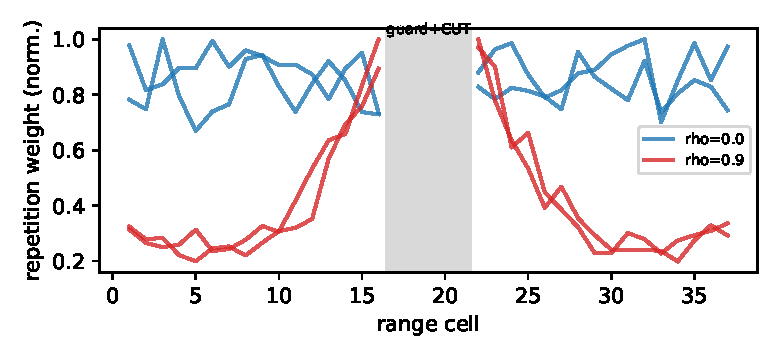
\includegraphics[width=0.62\linewidth]{figs/cfar_weights.pdf}
\caption{Learned repetition weights of the CFAR WOS-R (2 seeds per texture correlation), normalised to their maximum.}\label{fig:cfarw}\end{figure}

\begin{table}[t]\centering\small
\caption{B4: constant-false-alarm-rate (CFAR) detection in K-distributed clutter with range-correlated texture (AR(1) coefficient $\rho$), false-alarm probability $P_{fa}=10^{-4}$ calibrated per detector. Signal-to-noise ratio (SNR, dB) for detection probability $P_d=0.5$ with 0/2/4/8 interfering targets in the reference window (lower is better); learned detectors: mean of 2 seeds, trained with the same Neyman--Pearson objective.}\label{tab:b4}
\setlength{\tabcolsep}{4pt}\begin{tabular}{lr|cccc|cccc}\toprule
& & \multicolumn{4}{c|}{$\rho=0$} & \multicolumn{4}{c}{$\rho=0.9$}\\
Detector & Params & 0 & 2 & 4 & 8 & 0 & 2 & 4 & 8\\\midrule
OS-CFAR ($k{=}24$) & 0 & 15.46 & 16.41 & 17.33 & 19.91 & 14.43 & 15.30 & 16.27 & 18.75\\
GO-OS ($k{=}11$) & 0 & 15.76 & 16.63 & 17.50 & 20.09 & 14.91 & 15.72 & 16.50 & 18.85\\
WOS-R (32 repetitions) & 34 & 15.55 & \textbf{16.29} & \textbf{16.95} & \textbf{18.38} & 14.20 & \textbf{14.83} & \textbf{15.53} & \textbf{17.09}\\
MLP (log-equivariant) & 6\,337 & \textbf{15.22} & 17.64 & 19.37 & 22.69 & \textbf{13.86} & 15.92 & 17.57 & 20.35\\
Transformer (log-equivariant) & 5\,009 & 15.55 & $>30$ & $>30$ & $>30$ & 14.85 & $>30$ & $>30$ & $>30$\\
\bottomrule\end{tabular}\end{table}

\subsection{B5: robust aggregation}
Table~\ref{tab:b5} evaluates aggregation rules in federated training with 4 of 20 faulty nodes. No single-shot
aggregator survives all attacks: burst faults that persist over consecutive steps already drive the mean and both trimmed
means to chance accuracy (0.10), and the combined Gaussian-plus-burst fault does the same to the coordinate-wise (CW) median,
the adaptive minimax OWA (AMO, an OWA whose weights are chosen online from a precomputed minimax library) and the learned sorted-MLP aggregator; only centred clipping keeps a little above chance (0.14--0.18).
A learned MLP on sorted inputs standardised by the median and the median absolute deviation (MAD) (5\,569 parameters, trained on synthetic attack families) is no
exception: silent data corruption (SDC: sporadic huge
values from faulty hardware), which is not among its training families, drives it to 0.11, since nothing bounds the influence of an input
that leaves the training range. What
restores robustness is the \emph{cascade} structure of the thesis applied to the time$\times$node axes: a per-node
temporal median over the last 3 submissions, followed by nearest-neighbour mixing and a final order-statistic aggregator.
This ordinal cascade, with no trained parameters, has the best worst-case accuracy for $\alpha=1$ (0.753). Replacing its
last stage by the learned MLP improves the heterogeneous worst case ($\alpha=0.1$: 0.615 vs 0.535, driven by IPM) at a
small cost in the homogeneous case (0.740). The robustness comes from the rank cascade; the learned stage adds
accuracy only once the cascade has bounded the influence of the faulty inputs.

\begin{table*}[t]\centering\small
\caption{B5: Byzantine/fault-robust aggregation (Fashion-MNIST, $n{=}20$ nodes, $f{=}4$ faulty, 300 steps, mean of 2 seeds). Test accuracy under each attack with heterogeneous data (Dirichlet $\alpha{=}0.1$), and worst case over attacks for $\alpha\in\{1,0.1\}$. CW: coordinate-wise; Med$_t$3: per-node temporal median of the last 3 submissions; NNM: nearest-neighbour mixing \cite{allouah2023}; AMO: adaptive minimax ordered weighted average (OWA). Attacks: ALIE (``a little is enough''), IPM (inner-product manipulation), burst-8 (faults persisting 8 steps), SDC (silent data corruption). $^\dagger$AMO uses a precomputed library of 5 OWA weight vectors (minimax second-order cone program), no training.}\label{tab:b5}
\resizebox{\linewidth}{!}{\begin{tabular}{lr|ccccccc|cc}\toprule
& & \multicolumn{7}{c|}{$\alpha=0.1$} & \multicolumn{2}{c}{worst case}\\
Aggregator & Params & none & sign-flip & ALIE & IPM & burst-8 & SDC & Gauss+burst & $\alpha{=}1$ & $\alpha{=}0.1$\\\midrule
Mean & 0 & 0.814 & 0.414 & 0.787 & 0.789 & 0.100 & 0.100 & 0.100 & 0.100 & 0.100\\
CW median & 0 & 0.603 & 0.599 & 0.565 & 0.465 & 0.244 & 0.683 & 0.100 & 0.100 & 0.100\\
CW trimmed mean & 0 & 0.728 & 0.642 & 0.728 & 0.372 & 0.100 & 0.707 & 0.100 & 0.100 & 0.100\\
NNM + CW trim & 0 & 0.793 & 0.727 & 0.714 & 0.695 & 0.100 & 0.803 & 0.100 & 0.100 & 0.100\\
Centred clipping & 0 & 0.806 & 0.681 & 0.771 & 0.693 & 0.707 & 0.803 & 0.141 & 0.177 & 0.141\\
AMO (minimax OWA) & 0$^\dagger$ & 0.591 & 0.551 & 0.610 & 0.410 & 0.247 & 0.602 & 0.100 & 0.100 & 0.100\\
Med$_t$3 $\to$ AMO & 0$^\dagger$ & 0.576 & 0.502 & 0.527 & 0.264 & 0.542 & 0.548 & 0.539 & 0.691 & 0.264\\
Med$_t$3 $\to$ NNM $\to$ CW trim & 0 & 0.779 & 0.672 & 0.772 & 0.535 & 0.782 & 0.773 & 0.762 & \textbf{0.753} & 0.535\\
Sorted-MLP aggregator & 5\,569 & 0.673 & 0.646 & 0.718 & 0.380 & 0.101 & 0.113 & 0.100 & 0.100 & 0.100\\
Med$_t$3 $\to$ NNM $\to$ sorted-MLP & 5\,569 & 0.777 & 0.703 & 0.767 & 0.615 & 0.780 & 0.775 & 0.773 & 0.740 & \textbf{0.615}\\
\bottomrule\end{tabular}}\end{table*}

\subsection{Cost summary}
Table~\ref{tab:cost} pairs the best WOS-R model with the best network on each task. Parameter savings are 161$\times$ (1D),
186$\times$ (CFAR) and 1\,434$\times$ (images); multiplications drop from $6\cdot10^3$--$7\cdot10^4$ per sample to
0--8, replaced by a few hundred comparisons. The accuracy cost in distribution is 0.5--1.2\,dB; out of distribution the
sign flips. Wall-clock latency with generic PyTorch kernels does \emph{not} reflect these savings: sorting unfolded
windows is memory-bound and the bank evaluates $C$ chains sequentially, so WOS-R is 1.1--4.5 times slower than CNNs of
similar accuracy on a CPU. The operation counts, not this latency, are what a comparator implementation would exploit.

\begin{table*}[t]\centering\small
\caption{Cost summary: best WOS-R vs best network per task. Mults/Comps per output sample or pixel; ms: CPU latency (1 thread; 4096 samples in 1D, $512{\times}512$ in 2D) with generic PyTorch kernels.}\label{tab:cost}
\resizebox{\linewidth}{!}{\begin{tabular}{l|lrrrrr|lrrrr}\toprule
Task & WOS-R model & Params & Mults & Comps & ms & Score & Network & Params & Mults & ms & Score\\\midrule
B1 impulsive (NMSE dB) & WOS-R bank $C{=}8$ & 137 & 8 & 336 & 16.9 & -21.1 & CNN-L & 22\,081 & 21\,952 & 3.8 & -22.3\\
B1 OOD amplitude (NMSE dB) & WOS-R bank $C{=}8$ & 137 & 8 & 336 & 16.9 & -17.8 & CNN-L & 22\,081 & 21\,952 & 3.8 & -17.4\\
B3 BSD68 SP 50\% (PSNR) & Switching WOS-R $5{\times}5$ & 52 & 0 & 268 & 665.9 & 26.22 & DnCNN-M (10 layers, 32 ch) & 74\,593 & 74\,304 & 616.2 & 26.74\\
B3 BSD68 RVIN 40\% (PSNR) & WOS-R $5{\times}5$, 2 stages & 52 & 0 & 250 & 722.0 & 24.46 & DnCNN-M (10 layers, 32 ch) & 74\,593 & 74\,304 & 616.2 & 17.74\\
B4 CFAR, $\rho{=}0.9$, 8 interf.\ (SNR$_{50}$ dB) & WOS-R & 34 & 1 & 160 & -- & 17.09 & MLP & 6\,337 & 6\,208 & -- & 20.35\\
\bottomrule\end{tabular}}\end{table*}

\begin{figure*}[t]\centering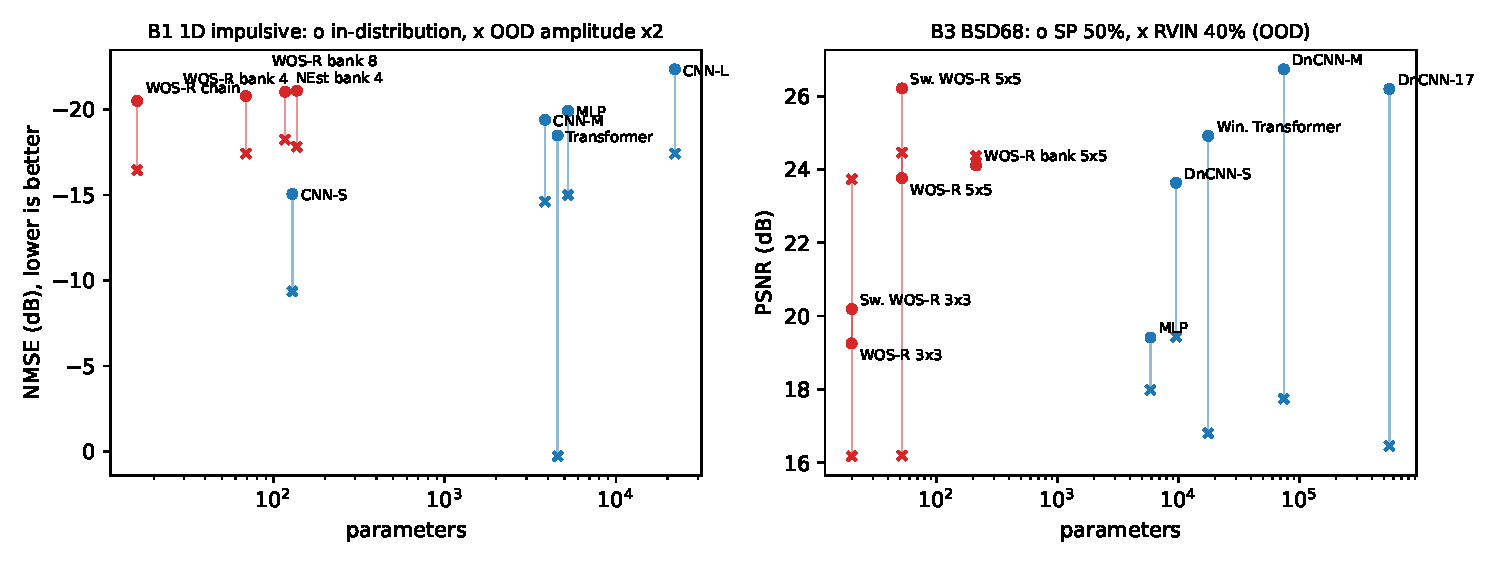
\includegraphics[width=0.95\linewidth]{figs/pareto.pdf}
\caption{Accuracy versus parameters (log scale). Red: order-statistic models; blue: networks. Vertical segments join
in-distribution (o) and out-of-distribution (x) scores of the same model: short segments mean robust models.}\label{fig:pareto}\end{figure*}


%=====================================================================================================
\section{Discussion}\label{sec:disc}
\paragraph{What the benchmark says.} Across the five problems the pattern is consistent. WOS-R is competitive in
distribution with networks two to four orders of magnitude larger whenever the contamination is impulsive or
heavy-tailed, and it is \emph{better} whenever the test distribution moves in a direction that a selection ignores:
larger impulse amplitudes (B1), a different impulse type (B3, RVIN), or a higher Gaussian level (B1, B3); the same
mechanism makes it the best detector in the presence of interfering targets (B4), which were present in training but
contaminate any smooth function of the reference cells. These are the directions in which a 1-Lipschitz, bounded-influence model cannot be surprised, whereas
networks trained by empirical risk minimisation have no such guarantee; the Transformer shows the most severe failures
(B1, B4). Conversely, WOS-R loses when the task requires averaging in distribution (Gaussian noise, $\approx2$\,dB), when the
contamination rate exceeds the design breakdown point (B1, $p=25\,\%$, $\approx3$\,dB), and, by construction, on the operators
outside the class $\mathcal O$ (B2): signed linear filters, non-increasing operators such as the top-hat, and point-wise
nonlinearities. Table~\ref{tab:decision} summarises the trade-off.

\begin{table}[t]\centering\small
\caption{When to use WOS-R (summary of B1--B5).}\label{tab:decision}
\begin{tabular}{p{0.44\linewidth}p{0.47\linewidth}}\toprule
WOS-R preferable & Network preferable\\\midrule
Impulsive/heavy-tailed noise, unknown amplitude or type & Gaussian noise at the training level\\
Interference-limited detection (CFAR) & Contamination rate above the design breakdown\\
Byzantine/fault-robust aggregation (as a cascade front-end) & Signed linear, non-increasing or level-dependent operators\\
$\le$\,200 parameters, $\le$\,8 multiplications, certified Lipschitz/breakdown & Highest in-distribution PSNR with GPU training\\
\bottomrule\end{tabular}\end{table}

\paragraph{Cascades as robust front-ends.} The federated experiment suggests the most practical use: a rank cascade
first bounds the influence of corrupted inputs, and a learned stage then adds accuracy (B5: 0.535$\to$0.615 worst-case
accuracy under heterogeneity). The same composition applies to images (a WOS-R front-end followed by a small CNN) and to
radar (WOS-R CFAR followed by a learned classifier). Because a WOS cascade is increasing and translation invariant,
any back-end that is 1-Lipschitz in $\ell_\infty$ preserves the end-to-end bound.

\paragraph{The 1993 question, revisited.} The thesis \cite{delrio1993} concluded that parameters acting only on the
\emph{index} of the selected sample (masks, ranks) cannot be adapted in a cascade, while parameters entering the
\emph{value} can. Repetition weights are index parameters, and exact WOS stages indeed have zero gradients almost
everywhere. The ramp resolves the dilemma by giving index parameters a value effect \emph{only during training}: the
gradient flows through the interpolation between rank neighbours, and the interpolation is removed at deployment. In
the identification task of the thesis, this raises the fraction of random cascades identified from 2--3 of 16 (NEst,
value parameters) to 9 of 16 (paired Wilcoxon $p=4.6\cdot10^{-8}$ over 3 seeds).

\paragraph{Hardware.} A deployed WOS-R stage needs a sorting network and a running sum of integer repetitions
(Prop.~\ref{prop:thr}(iii)); a bank adds $C$ multiplications per sample. This maps to comparator-only logic on field-programmable gate arrays (FPGAs) and
low-power digital signal processors (DSPs), the setting in which stack and weighted-median filters were originally implemented \cite{wendt1986stack,yin1996}.

\section{Limitations}
All training ran on a 2-core CPU. Image models use a single training seed and at most 3\,000 steps, so the CNN and
Transformer baselines are under-trained relative to published GPU models; we mitigate this by reporting their failure
modes only where they persist across model sizes. The CFAR study uses simulated K-distributed clutter with an AR(1)
texture model, and the federated study a small CNN on Fashion-MNIST \cite{xiao2017fmnist} with 20 nodes. Latency is
measured with generic PyTorch kernels (sorting by \texttt{torch.sort} on unfolded windows), which favour convolutions;
the multiplication and comparison counts are the hardware-relevant quantities, and a sorting-network or comparator
implementation remains to be built. Finally, the ramp gives exact gradients of a relaxed model but no guarantee of
finding the global optimum: a two-stage chain represents the opening exactly, yet ramp training does not find it
(Table~\ref{tab:b2}), and random cascades are identified in 9 of 16 cases.

\section{Conclusion}
We have shown that weighted order statistic cascades, a 40-year-old family of nonlinear filters, become trainable with a
simple device---a ramp relaxation used only during training---and that the resulting models keep their guarantees at
deployment. With tens to a few hundred parameters and almost no multiplications, they match or approach CNNs, MLPs
and Transformers that are two to four orders of magnitude larger on impulsive restoration and detection, and order-statistic models are
the most robust in every out-of-distribution test that changes the amplitude, the impulse type or the noise
level---though not when the contamination rate exceeds their design breakdown point. Their limits are equally clear: they are not
universal approximators and should be combined with linear or learned stages when the target is outside the class of
increasing, translation-invariant operators. Learned switching detectors, hybrid WOS--linear layers and comparator
hardware are natural next steps.

\paragraph{Historical note.} The structures studied in \cite{delrio1993} (rank-order filters (ROF), LL-filters and the NEst structure
$y=\sum_k|h_k|(z+b)_{(k)}$) were adapted sample by sample with LMS and implicit-function derivatives. Re-implemented
with exact reverse-mode gradients, the 1993 NEst cascade reaches the noise floor on the thesis' own example in 7\,s
instead of 20\,s, but identifies only 2--3 of 16 random cascades. Repetition weights with ramp training identify 9 of 16.

\bibliographystyle{unsrtnat}
\bibliography{refs}

\appendix
\section{Abbreviations}\label{app:abbr}
\begin{center}\small
\resizebox{\linewidth}{!}{\begin{tabular}{@{}ll@{\qquad}ll@{}}\toprule
ALIE & ``a little is enough'' attack & MAD & median absolute deviation\\
AMF & adaptive median filter & Med$_t$3 & per-node temporal median of the last 3 updates\\
AMO & adaptive minimax OWA aggregator & MLP & multilayer perceptron\\
BN & batch normalisation & MSE & mean squared error\\
BSD68 & Berkeley segmentation dataset, 68 test images & NEst & 1993 rank structure $\sum_k|h_k|(z+b)_{(k)}$\\
CClip & centred clipping & NMSE & normalised mean squared error\\
CDF & cumulative distribution function & NNM & nearest-neighbour mixing\\
CFAR & constant false-alarm rate & OOD & out of distribution\\
CNN & convolutional neural network & OS-CFAR & order-statistic CFAR\\
CUT & cell under test & OWA & ordered weighted average\\
CW & coordinate-wise & $P_d$, $P_{fa}$ & detection / false-alarm probability\\
DnCNN & denoising CNN \cite{zhang2017dncnn} & PSNR & peak signal-to-noise ratio\\
DSP & digital signal processor & ROF & rank-order filter\\
FFN & feed-forward network & RVIN & random-valued impulse noise\\
FL & federated learning & SDC & silent data corruption\\
FPGA & field-programmable gate array & SNR, SNR$_{50}$ & signal-to-noise ratio (at $P_d=0.5$)\\
GO/SO-OS & greatest-of/smallest-of OS-CFAR & SP & salt-and-pepper noise\\
IPM & inner-product manipulation attack & SSIM & structural similarity index\\
K-distr. & compound-Gaussian sea-clutter model & STE & straight-through estimator\\
LMS & least mean squares & SVM & support vector machine\\
Mults/Comps & multiplications/comparisons per output & WOS & weighted order statistic\\
 & & WOS-R & WOS trained with ramps, deployed exact\\
\bottomrule\end{tabular}}\end{center}

\section{Additional tables}\label{app:tables}
\begin{table*}[t]\centering\small
\caption{B3: blind impulse denoising on Set12, peak signal-to-noise ratio (PSNR, dB; higher is better) / structural similarity (SSIM). Training: salt-and-pepper (SP) with density $\sim U[0.1,0.6]$. Out of distribution (OOD): SP 70\,\%, random-valued impulse noise (RVIN). AMF: adaptive median filter; switching: WOS-R applied only to pixels that are an extreme of their $3{\times}3$ window. Mults and comparisons per pixel; latency in ms for a $512{\times}512$ image (1 CPU thread). Best per column in bold.}\label{tab:b3set12}
\resizebox{\textwidth}{!}{\begin{tabular}{lrrrr|cccc|cc}\toprule
Model & Params & Mults & Comps & ms & SP 10\% & SP 30\% & SP 50\% & SP 70\% & RVIN 20\% & RVIN 40\%\\\midrule
Median $3{\times}3$ & 0 & 0 & 36 & 52 & 29.02/0.888 & 22.31/0.713 & 14.87/0.279 & 9.74/0.076 & \textbf{27.40}/0.848 & 22.41/0.614\\
Median $5{\times}5$ & 0 & 0 & 125 & 149 & 26.38/0.809 & 25.05/0.785 & 21.63/0.682 & 13.63/0.245 & 25.77/0.795 & 23.95/0.727\\
Adaptive median (AMF, 7) & 0 & 0 & var. & 386 & 33.09/0.957 & 29.15/0.925 & 25.87/0.864 & 20.11/0.674 & 21.63/0.541 & 16.59/0.273\\
WOS-R $3{\times}3$, 2 stages & 20 & 0 & 72 & 178 & 28.07/0.868 & 25.73/0.829 & 19.39/0.598 & 11.92/0.163 & 27.14/0.851 & 24.35/0.742\\
WOS-R $5{\times}5$, 2 stages & 52 & 0 & 250 & 722 & 27.44/0.842 & 26.19/0.820 & 23.79/0.770 & 15.86/0.453 & 26.78/0.829 & \textbf{24.85}/0.777\\
WOS-R bank $C{=}4$ ($3{\times}3$) & 85 & 4 & 288 & 489 & 27.13/0.847 & 25.77/0.815 & 20.70/0.576 & 13.47/0.176 & 26.31/0.833 & 24.02/0.740\\
WOS-R bank $C{=}4$ ($5{\times}5$) & 213 & 4 & 1\,000 & 2806 & 27.31/0.840 & 26.23/0.821 & 24.15/0.764 & 16.82/0.403 & 26.61/0.827 & 24.74/0.777\\
\quad ablation: bank $C{=}4$ ($3{\times}3$), ramp only & 85 & 4 & 288 & 489 & 27.79/0.860 & 25.98/0.822 & 20.42/0.571 & 13.19/0.170 & 26.84/0.845 & 24.24/0.744\\
\quad ablation: bank $C{=}4$ ($5{\times}5$), ramp only & 213 & 4 & 1\,000 & 2806 & 27.48/0.845 & 26.33/0.825 & 24.12/0.768 & 16.56/0.398 & 26.75/0.832 & 24.80/0.779\\
Switching WOS-R $3{\times}3$ & 20 & 0 & 90 & 240 & 32.01/0.951 & 27.88/0.912 & 20.19/0.670 & 12.49/0.198 & 21.61/0.538 & 16.68/0.272\\
Switching WOS-R $5{\times}5$ & 52 & 0 & 268 & 666 & 31.27/0.943 & 28.99/0.924 & 26.03/0.870 & 18.43/0.629 & 21.54/0.532 & 16.69/0.269\\
Switching WOS-R bank $C{=}4$ ($3{\times}3$) & 85 & 4 & 306 & 726 & 30.86/0.907 & 28.17/0.865 & 22.10/0.620 & 14.89/0.226 & 21.47/0.526 & 16.64/0.269\\
MLP $5{\times}5$ & 5\,889 & 5\,760 & 0 & 129 & 30.41/0.880 & 24.56/0.637 & 19.69/0.396 & 15.64/0.214 & 21.84/0.492 & 18.11/0.314\\
DnCNN-S (6 layers, 16 ch) & 9\,585 & 9\,504 & 0 & 44 & 29.57/0.878 & 26.49/0.744 & 23.82/0.600 & 20.23/0.417 & 23.87/0.622 & 19.66/0.428\\
DnCNN-M (10 layers, 32 ch) & 74\,593 & 74\,304 & 0 & 616 & \textbf{33.64}/0.949 & \textbf{30.10}/0.883 & \textbf{26.87}/0.766 & \textbf{22.00}/0.536 & 22.38/0.520 & 18.26/0.338\\
DnCNN-17 (BN, 64 ch) & 556\,097 & 554\,112 & 0 & 3065 & 29.95/0.882 & 28.95/0.812 & 26.11/0.704 & 21.41/0.505 & 21.50/0.470 & 17.37/0.300\\
Window Transformer & 17\,697 & 25\,152 & 0 & 1247 & 30.23/0.914 & 27.98/0.834 & 25.05/0.701 & 20.72/0.474 & 20.77/0.450 & 17.40/0.300\\
\bottomrule\end{tabular}}\end{table*}

\section{Hyper-parameters}\label{app:hyper}
\begin{itemize}
\item \textbf{WOS-R}: repetition weights $w=\mathrm{softplus}(\alpha)$, initialised at $\approx1$; quantile $r=\sigma(\rho)$, initialised at $0.5$;
  training at $\beta=1$ for chains and with $\beta$ annealed linearly from 1 to 0 over the first 70\,\% of the steps for banks,
  deployment at $\beta=0$; Adam, $\eta=0.03$, cosine decay to $5\%$.
  1D: windows of 7 samples, 2 stages per chain, banks of $C\in\{1,4,8\}$ chains with affine mix.
  2D: $3{\times}3$ or $5{\times}5$ windows, 2 stages, $C\in\{1,4\}$.
\item \textbf{1D baselines}: residual CNN-S (3 layers, 4 channels, kernel 5), CNN-M (4 layers, 16 channels, kernel 7),
  CNN-L (5 layers, 32 channels, kernel 7); MLP on a 15-sample window ($15{\to}64{\to}64{\to}1$, residual);
  Transformer (conv embedding to $d{=}16$, 2 encoder layers, 2 heads, feed-forward network (FFN) width 32, full attention, residual).
  Adam, $\eta=2\cdot10^{-3}$, 3000 steps, batch 32 crops of 256 samples.
\item \textbf{2D WOS-R}: chains of 2 stages on $3{\times}3$ or $5{\times}5$ windows; banks of 4 such chains; switching
  variants apply the model only where the centre pixel equals the minimum or maximum of its $3{\times}3$ window (18
  extra comparisons per pixel) and pass the input through elsewhere.
\item \textbf{2D baselines}: DnCNN-type residual networks, $3{\times}3$ convolutions: S (6 layers, 16 channels) and
  M (10 layers, 32 channels) without batch normalisation; DnCNN-17 (17 layers, 64 channels, batch normalisation, the
  original design \cite{zhang2017dncnn}; the variant without batch normalisation did not train); MLP on a $5{\times}5$ neighbourhood; window Transformer (conv embedding to $d{=}32$,
  2 blocks of $8{\times}8$ window attention, the second shifted, 4 heads, FFN 64). Adam, $\eta=10^{-3}$, 3000 steps
  (2000 for DnCNN-17 and WOS-R), batches of 16 patches of $48{\times}48$ from the 400 BSD training images, with
  random rotations and flips. A single training seed per model (CPU budget).
\item \textbf{B2 coverage}: input i.i.d.\ $U[-5,5]$, 64 sequences of 2\,048 samples, additive uniform noise at 35\,dB
  SNR; 3\,000 steps, batches of 16 crops of 256 samples; metric: NMSE of the deployed model minus the NMSE of the true
  operator applied to the noisy input (the floor). Models: WOS-R chain ($2{\times}7$), WOS-R bank $C{=}4$, NEst bank
  $C{=}4$, MLP (window 15), CNN-M, Transformer, as in B1.
\item \textbf{B4 CFAR}: 32 reference cells (16 leading, 16 lagging), 2 guard cells per side; K-distributed clutter with
  shape $\nu=2$, scene power uniform in $\pm20$\,dB, and Gaussian-copula AR(1) texture with coefficient $\rho\in\{0,0.9\}$
  along range; detectors act on
  $\log$ reference cells and output a log-threshold; training: 800 Adam steps of the Neyman--Pearson Lagrangian
  (sigmoid detection surrogate, temperature 0.25, quadratic penalty on $\log P_{fa}$ above $10^{-4}$), with 0/2/4/8
  interferers (20\,dB above the local clutter) and target SNR uniform in 10--20\,dB; evaluation: threshold scale
  calibrated on $4\cdot10^5$ clutter-only cells, $P_d$ on $10^5$ cells per SNR on a 5\,dB grid from 5 to 30\,dB, SNR at
  $P_d=0.5$ by linear interpolation. MLP: $32{\to}64{\to}64{\to}1$ on mean-removed logs; Transformer: $d{=}16$, 2 layers, 2 heads,
  learned positions, mean pooling.
\item \textbf{B5 aggregation}: Fashion-MNIST, small CNN, 20 nodes of which 4 faulty, Dirichlet label split
  $\alpha\in\{1,0.1\}$, worker momentum 0.9, 300 steps, learning rate 0.08; attacks: sign-flip, ALIE \cite{baruch2019},
  IPM \cite{xie2019ipm}, burst faults on 8 consecutive steps, SDC \cite{dixit2021sdc}, Gaussian plus burst. Sorted-MLP
  aggregator: per coordinate, sort the $n$ values, standardise by median and MAD, MLP $20{\to}64{\to}64{\to}1$
  (5\,569 parameters), trained on synthetic attack families to output the honest mean.
\item \textbf{Classical}: median, adaptive median filter (Hwang--Haddad, maximum window 7) \cite{hwang1995}, OS-CFAR, GO-OS,
  coordinate-wise median and trimmed mean.
\end{itemize}
\end{document}
